%
% File eamt18.tex
%

\documentclass[11pt]{article}
\usepackage{cs501R}
\usepackage{times}
\usepackage{url}
\usepackage{latexsym}
\usepackage[small,bf]{caption} % added MLF 20171211
\setlength\titlebox{6.5cm}    % Expanding the titlebox
%%% YOUR PACKAGES BELOW THIS LINE %%%

%% MJM

\title{Movies and Actors Network: PageRank}

\author{\\Marta Campagnoli\\
  Data Science and Economics\\
  Algorithms for Massive Data\\
  ID 928635\\
  {\tt marta.campagnoli@studenti.unimi.it}}

\date{}

\begin{document}
\maketitle


\section{Introduction}

The following report describes the process used in order to analyze the IMDB dataset of visual media with the aim to extract a network of movies and actors, where two movies are linked through an edge if they share at least an actor in their cast, with the final goal to classify the importance of each node through a PageRank algorithm designed for Big Data. Code for this project has been written and compiled in Python 3; to make sure the results of the processing were correct, a sample network has been also visualized through Gephi. The PageRank algorithm has been run using Spark on Google Colab.

Before explaining my work, I acknowledge that this project has been run on a machine with severe hardware limitations. Some of the steps taken, such as limiting the data the algorithms have been tested on and creating ausiliary files in order to work with edges, could be better dealt with on a better performing machine.

\section{Methodology}

The project has been carried out in three main steps: preprocessing the data and building the dataset, creating the edge files to use in the algorithm, and running the algorithm on the data.
The PageRank algorithm is a topic discussed during both class in the course and tutoring; in the project, I tried to adapt the proposed code for the network and edges I built in the processing phase.

\subsection{Dataset: chosen data and preprocessing}

The IMDB dataset proposed for the project is divided in 5 parts, of which 4 were used during the project: to build the dataset and for the first part of the preprocessing process I used three of them, specifically the ``title.basics" file containing information about movies, tv shows and other kind of audio-visual media such as videogames, the ``title.principals" file containing the main group of people that worked in each piece (not only actors, but also directors, main assistants and others) and the``name.basics" files containing information for each person credited for work on IMDB. While in theory the ``title.principals" file would be sufficient to create edges between works, merging the three files to create a dataset was useful to filter out redundant data that would make the network meaningless - or,in other words, a network of each person that has worked in any capacity in any work cited on IMDB.\\

As a first step, I worked on the ``title.principals" file in order to extract a subset of the data in which only actors appeared. 
Secondly, from the ``title.basics" file I filtered out all records that didn't contain a movie (for cinema or tv release).
Then,  from``name.basics" I once again extracted records for actors only. 
By performing an inner join on the first and third file by actor ID (column ``nconts"), I created a dataset where each row contained an actor (by both name and identifying code) and a piece of media they worked in (by identifying code), so that for each actor I now had a record for each movie they acted in. By performing another inner join of the resulting dataset with the filtered "title.basics" file by movie ID (column ``tconst"), I then created the complete dataset containing each movie by name and ID code  in each containing in each row a different actor (by name and ID) that acted in that movie, with additional info for later use.\\

After filtering out redundant columns, I performed a groupby count by actor name in order to filter out actors with a count of 1 (with only one acting credit), because those records aren't useful to create edges, as the actor wouldn't connect any two movie. 

Finally, in order to correctly apply the next steps in the project, I sorted the data by movie title and created the dataset as is.

\subsection{Testing the dataset: building a small network}

In order to build the network, four functions have been created:
\begin{itemize}
  \item the ``indeces" function, used later on to associate each movie to an inde;
  \item the ``listcreation1" and ``listcreation2" functions, which respectivelly create two lists of movie name-actor name tuples and two lists of movie index-actor name tuples;
  \item the ``edgelistdirected" function, used to automatically create edges from two lists of movie-actors tuples.
\end{itemize}

As previously stated, because of the limits of the hardware I worked on, I decided to test each step on a very small dataset. This was done by choosing a subset containing movies by only two actors based on previous personal knowledge: Taika Waititi and Jemaine Clement are two actors from Aotearoa, New Zealand who only ever acted on one movie together, ``What We Do In The Shadows" (2014), so the node representing the movie is expected to have higher centrality in the network and higher PageRank, since it will be connected to each movie in the network.\\

\begin{figure}[h!]
\centering
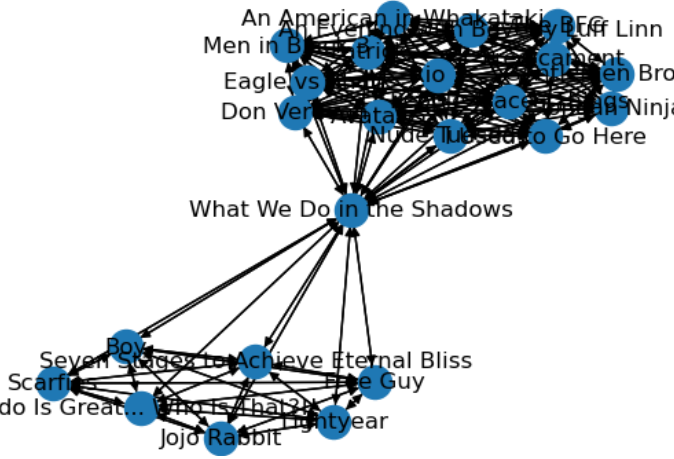
\includegraphics[height=5cm]{py3.png}
\caption{Network visualized through Networkx.}
\label{fig:network1}
\end{figure}

Starting from this assumption, I proceeded to filter the dataset to get only movies starring the chosen actors, to create an auxiliary column of movie-actor tuples, to apply the ``listcreation1" functions on the dataset two extract the column in two lists, and to apply the ``edgelistdirected" function on the two lists in order to create an edges file. A first weakness of the process emerges from this step: the ausiliary movie-actor column in the dataset needs to be created everytime a new edges file is needed for a certain dataset, because saving the dataset in .csv format will turn each tuple in an object unreachable by index, which will stop the ``edgelistdirected" functions from working. 

Using the Networkx package, with title names from the data as nodes, and the edges file from the previous step as files, I visualized the network both via Networkx (figure 1) and Gephi (figure 2).



\begin{figure}[h!]
\centering
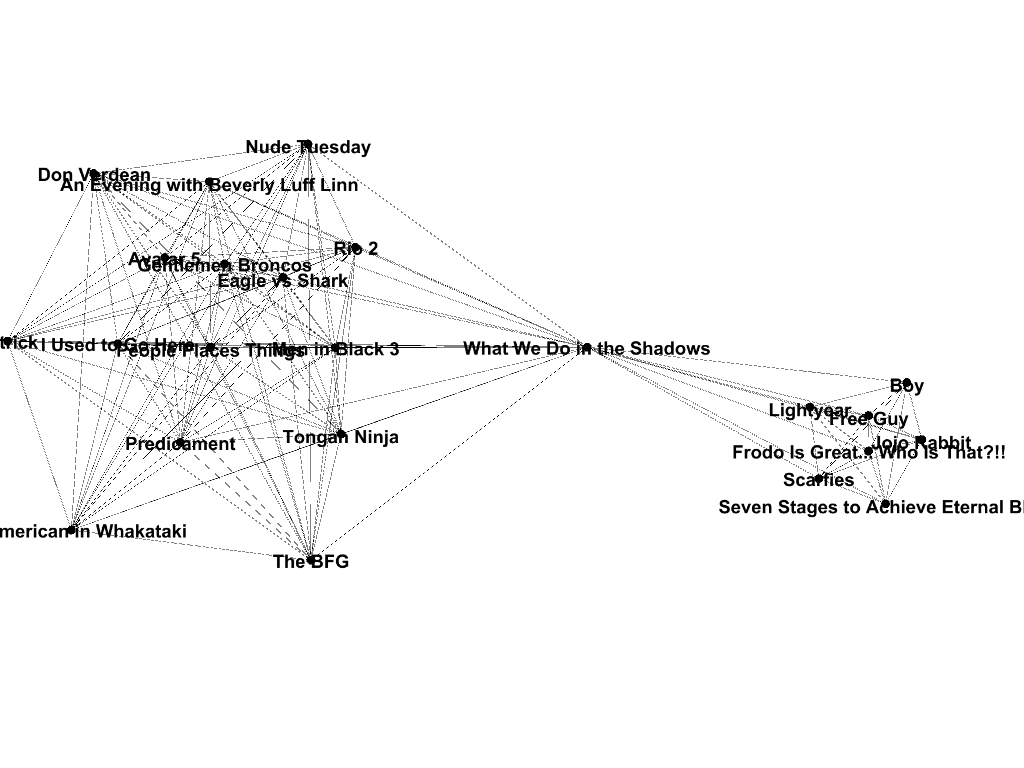
\includegraphics[height= 6 cm]{taikajem.png}
\caption{Gephi-Force Atlas Layout.}
\label{fig:netowrk2}
\end{figure}

The visualization shows that the central node is indeed ``What We Do In The Shadows". In order to be able to later compare results, I also ran the built in Networkx pagerank function on the graph; the highest result is also for the aforementioned movie, with value of 0.07467.

\subsection{Restricting the dataset: another step in processing}

As a last step to create a restricted dataset whose dimension could allow the creation of the edges locally, I performed a last step in processing. 
After filtering out documentaries through string manipulation on the ``genres" column, I performed an inner join of the dataset with the ``title.akas" file containing release regions in order to filter out duplicates by keeping only movies by their USA release title; I then created three separate datasets, one for the years 2017 onward, one for the years 2020-2021 and one for 2020 only. 
The 2020-2021 was the one used, comprising approximately 3600 nodes, along with the sample network of two actors, in the next steps.

\subsection{Indexing: creating edges for Spark and MapReduce}
\

I acknowledge the next paragraph describes an auxiliary process that could be avoided when using well-performing hardware, simply creating network edges from the dataset in a Google Colab environment and using it via SparkContext to run the PageRank algorithm; instead, I had to create a brief alternative solution to obtain an edges file that I could feasibly use.\\

After repeating the filtering out of actors with one movie only to avoid discrepancies in the number on nodes and edges on the 2020-2021 network, for both this graph and the network of two actors I applied the ``indeces" function, now mapping the title names to indeces, created a movie index-actor name column, and created a file of edges through the ``listcreation2" and ``edgelistdirected" functions. The edges are now using indeces instead of movie names, and are saved in .json files for later use. 

\subsection{PageRank: Spark and MapReduce}

While the process along with the results will be better explained in the next paragraph, I briefly specify that the chosen algorithm for Link Analysis on the dataset was PageRank; the code has been implemented in SparkContext with a MapReduce algorithm for scaling up replicability. 

\section{Results and Analysis}

\subsection{PageRank: experiments and results}

As stated in the introduction, the algorithm as been ran by adapting the solutions seen during the course and tutoring hours. 
Both algorithms are run through Spark using MapReduce, for replicability on large scale data. 
Both solutions have been tested on both the small network and the 2020-2021, and while not all of them have worked, I include a discussion of all results in the report.
All experiments have started by initializing a SparkContext and creating a Spark object in Google Colab, using the json files obtained in the previous steps to create an edge file then parallelized through Spark. From the parallelized RDD edgefile I used Map functions to count nodes, compute outdegrees, set the vector of initial probabilities for each node, create the connection matrix and finally apply the MapReduce algorithm.

The core code of the two sets of experiments is the same, if note for variables names; the difference comes from the stopping rule of the algorithm.

The first set of experiments doesn't set a stopping rule, but runs the algorithm on a for loop set on a range. This algorithm works both on the small network (50 iterations) confirming the results obtained with the Networkx built it function - with node 22 corresponding to ``What We Do In The Shadows" having the highest rank of 0.07434 - and on the bigger network of 8641 nodes. In this case, however, the high node has page rank value of 0.00205; it needs to be considered that the vector of initial probabilities is initialized with each value set at 0.00011819 - each probability is in fact equal to \begin{equation}
    1/ number of nodes
\end{equation}
\vspace{1mm}\\

We know the algorithm converges to the true value of PageRank, so setting an high enough number of iterations will ensure that our results will be tending to the correct set of values, but this could also lead to wasting computational and time resources because it could be that we need less iterations than the ones we set.
In fact, when running a second set of experiments by using the Euclidean distance between the old and new value of the page rank as a stopping rule, we find that the algorithm for the small network stops after 17 iterations; in this case, however, the algorithm doesn't work on the 2020-2021 dataset because an error in the computation of the Euclidean distance itself; as stated, I decided to keep this information in the report to acknowledge that my project would need further work to ensure replicability and solve this issue. 

Later analysis in order to find a solution showed that a possible reason is a slight discrepancy between index values and the actual number of nodes in the network; indexing is done before the creation of edges, and despite filtering on the dataset, some movies appear to have no edges, so not all indexed values appear in the edges file; I assume that this causes a difference between the lenght of the initial array of probabilities and the first array of computed pagerank values, which will have less elements. When not computing the distance, this doesn't cause an issue in the computation, but only a small error in the initial probabilities, which are slightly lower than the correct value; however, this should be compensated by the high number of iterations set in the algorithm. As for the network of two actors, it's a controlled experiment where each indexed movie surely has an edge, so all algorithms work and the initial probabilities are set to the correct value.

The error in filtering could be caused by the fact that the data contains a lot of imprecise records, which would require additional information or processing; the``genre" column, as an example, is a string that should be worked via text processing to extract via regex each of the possible values, as the movie category contains in fact elements such as documentaries or biography. As another example, a lot of movies are stored twice or more times for each geographical zone they have been released in, but there is no data on the actual region of release, giving way to a number of duplicate records.
Unfortunately, because of time constraint, I was ultimately unable to completely clean the dataset, and fixing this issue is a question that remains unsolved.
On a different perspective, the problem could be solved by finding a different solution for the creation of edges and indexing. 

Lastly, although this experiment failed on the 2020-2021 network, I still decided to apply the algorithm for PageRank with Taxation on the small network with Euclidean distance as a stopping rule. Once again, results are similar but the algorithm stops in only 6 iterations. However, the nature of the network is such that applying taxation could be unnecessary; each link exists in two directions, so it's impossible to have dangling nodes or spider traps. However, although it's extremely unlikely for a group of movies to coincidentally only share actors among themselves and not having any connection to the main component, we cannot completely exclude this possibility and implementing and solving the issue of the Euclidean distance computation for this particular network could be useful. 

Figure 3 shows the network of two actors whose nodes have been colored with respect to the pagerank values obtained in the first experiment, with a color grading going from dark green (lowest values) to yellow (highest values). The result for the experiments ran on the algorithm using Euclidean distance as stopping rule where the same, so the graphs are not shown here as they are the same.

\begin{figure}[h!]
\centering
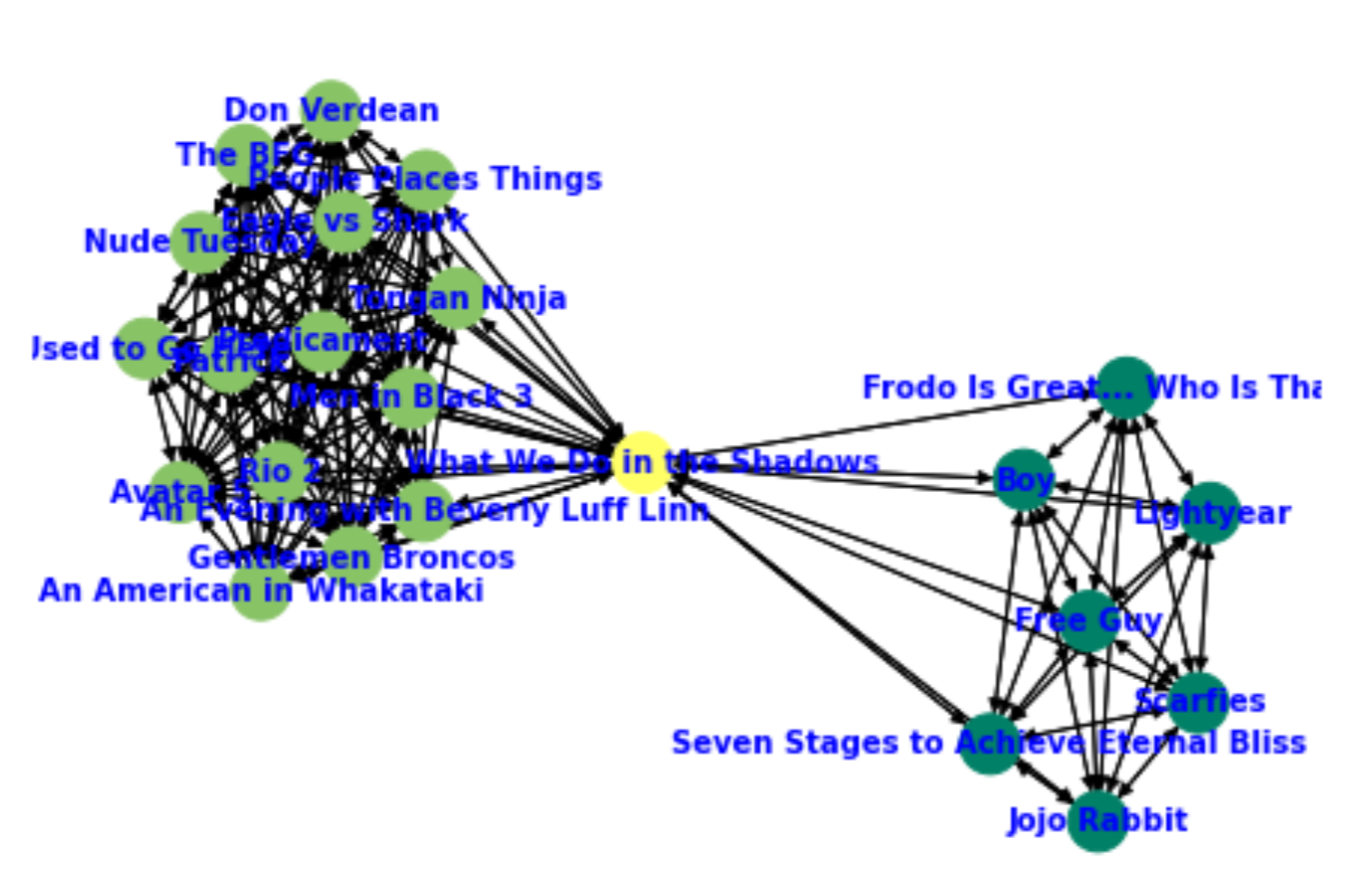
\includegraphics[height= 5 cm]{pagerankgraph.png}
\caption{Two actors network, nodes colored by pagerank value}
\label{fig:network3}
\end{figure}

\section{Conclusions}

The choice of implementing PageRank for link analysis on the network instead of another algoruthm came from the assumption that the more actors a movie shares with other works, the more important it could be in terms of notoriety in real life, but also in a network where links are created among nodes if they share an actor: the more actors shared, the more links connected to the node.
In fact PageRank is an algorithm based on ``random surfing", or the idea that a``surfer" will randomly follow a path given the links available from their starting point and they will keep "surfing" until the algorithm stops. The starting probabilities for each of the nodes are all equal, and as the algorithm converges, the higher the number of links leading to a node, the higher the final value of the pagerank associated to that node.

In this case, the more links reaching a movie because it shares actors with other works, and in turn, the more movies said actors have starred in, the higher the final value of the probability of the "random surfer" being in the node at the end of the process will be; however, when working in the 2020-2021 network, we have seen that the low value of the starting probability for each node in a huge network and the high number of nodes has lead to a very low value of pagerank for the node with highest result. While this could be coherent with a very low starting value of probability, I also ask myself if another algorithm would be more appropriate for this real life case. 

While the real life assumption that a ``star ridden" movie will have more exposure because of the actors' notoriety, this isn't reflected in the network because edges are not weighted and each has the same value, so the algorithm will only compute values based on the number of links and consequent outdegrees on which the connection matrix is based; potentially, a movie could very well share a large number of actors with others, with none of the actors being well known - in fact, some actors have tens or hundreds of credits for playing minor roles, but their edges will carry the same value (if not more) than those of an extremely famous actor with less credits.

Additionally, there are a number of variables that it wasn't possible to address in this project, both because of its scope and time constraints, and the nature of the data.

Among these, we can quote that the IMDB dataset has no data on the nationality or language of the movie, but only on whether movies were released in the US, and the importance of a movie can be better assessed when concentrating on a regional scope. 
So while one of the iterations of the algorithm worked on both networks it was tested on, better solutions could be found to address this particular case. So while the algorithm works, it could be that the result is mostly theoretical, unless used on a very controlled case for specific subsets of movies or actors.

On a more technical level, issues to address are the ability to store the lists of movie-actors tuples without having to create them each time edges for a specific network subset have to be generated; consequently making the generation of the tuple lists and edges into a single function routine; the ability to avoid the generation of an auxiliary edges file, but directly using the list in output from the ``edgelistdirected" function as an input for the connection matrix in Spark.\vspace{30mm}\\

\
\
I declare that this material, which I now submit for assessment, is entirely my own work and has not been taken from the work of others, save and to the extent that such work has been cited and acknowledged within the text of my work. I understand that plagiarism, collusion, and copying are grave and serious offences in the university and accept the penalties that would be imposed should I engage in plagiarism, collusion or copying. This assignment, or any part of it, has not been previously submitted by me or any other person for assessment on this or any other course of study.




\end{document}
